% =============================================================
%  ICRA 2027 submission (IEEEtran, conference, up to 8 pages)
%  Skill-Library-Guided Coevolution of Policy and Environment (SCOPE)
%  Compile: pdflatex main -> bibtex main -> pdflatex x2
%  INTEGRITY:
%   - Numbers marked "preliminary" are single-seed placeholders and
%     must be replaced by multi-seed, four-arm results before submission.
%   - [TODO] marks cells/figures to be filled from completed experiments.
% =============================================================
\documentclass[conference]{IEEEtran}
\IEEEoverridecommandlockouts

\usepackage{amsmath,amssymb,amsfonts}
\usepackage{algorithm}
\usepackage{algpseudocode}
\usepackage{graphicx}
\usepackage{booktabs}
\usepackage{xcolor}
\usepackage{multirow}
\usepackage[hidelinks]{hyperref}

\newcommand{\feasible}{\mathrm{feasible}}
\newcommand{\realized}{\mathrm{realized}}
\newcommand{\lv}{\mathrm{lv}}
\newcommand{\bcount}{n_{\mathrm{b}}}
\newcommand{\Wprobe}{\mathcal{W}_{\mathrm{probe}}}
\newcommand{\Dt}{\mathcal{D}_t}
\newcommand{\reasy}{r_{\mathrm{easy}}}
\newcommand{\rhard}{r_{\mathrm{hard}}}
\newcommand{\todo}[1]{\textcolor{red}{[TODO: #1]}}

\newtheorem{problem}{Problem}

\begin{document}

\title{Learnability from a Skill Library:\\
An LLM-Driven Environment Curriculum for\\ Zero-Shot Robot Policy Generalization}

\author{\IEEEauthorblockN{Anonymous Author(s)}
\IEEEauthorblockA{Affiliation (placeholder)\\
\texttt{email@placeholder}}}

\maketitle

\begin{abstract}
LLM-based methods can automatically construct diverse robotic training
environments, offering a promising avenue for improving policy generalization.
However, these methods typically assess generated environments through the
policy's current task performance, making it difficult to identify which
environments can further expand its capabilities. As a result, the generated
distribution may fail to keep pace with the policy's evolving learning needs.
To address this limitation, we propose \textbf{SCOPE}
(\textbf{S}kill-Library-Guided \textbf{CO}evolution of \textbf{P}olicy and
\textbf{E}nvironment), a closed-loop framework that couples latent-skill policy
learning with LLM-based evolution of programmatic training environments. At
each evolution cycle, task outcomes across the updated skill library reveal
capability coverage and characterize the learnability of candidate environments
relative to the policy's current capabilities. This feedback guides LLM-based
evolution of the environment-generator program, while interaction-based
validation selects the generator that defines the next training distribution.
We evaluate SCOPE on obstacle-constrained Push-T manipulation and navigation
across multiple unseen environment distributions. Across both tasks, SCOPE
achieves stronger zero-shot generalization than training distributions that are
manually designed, statically generated by an LLM, or evolved using aggregate
task-performance feedback. Analyses of skill-conditioned trajectories and
coevolution dynamics further reveal complementary behaviors and substantiate
the role of skill-library-relative feedback in training-distribution evolution.
Together, these results establish the learned skill library as an effective
feedback interface between policy learning and environment evolution.
\end{abstract}

\begin{IEEEkeywords}
Curriculum learning, environment generation, large language models, zero-shot
generalization, robotic manipulation, robot navigation.
\end{IEEEkeywords}

\begin{figure}[t]
\centering
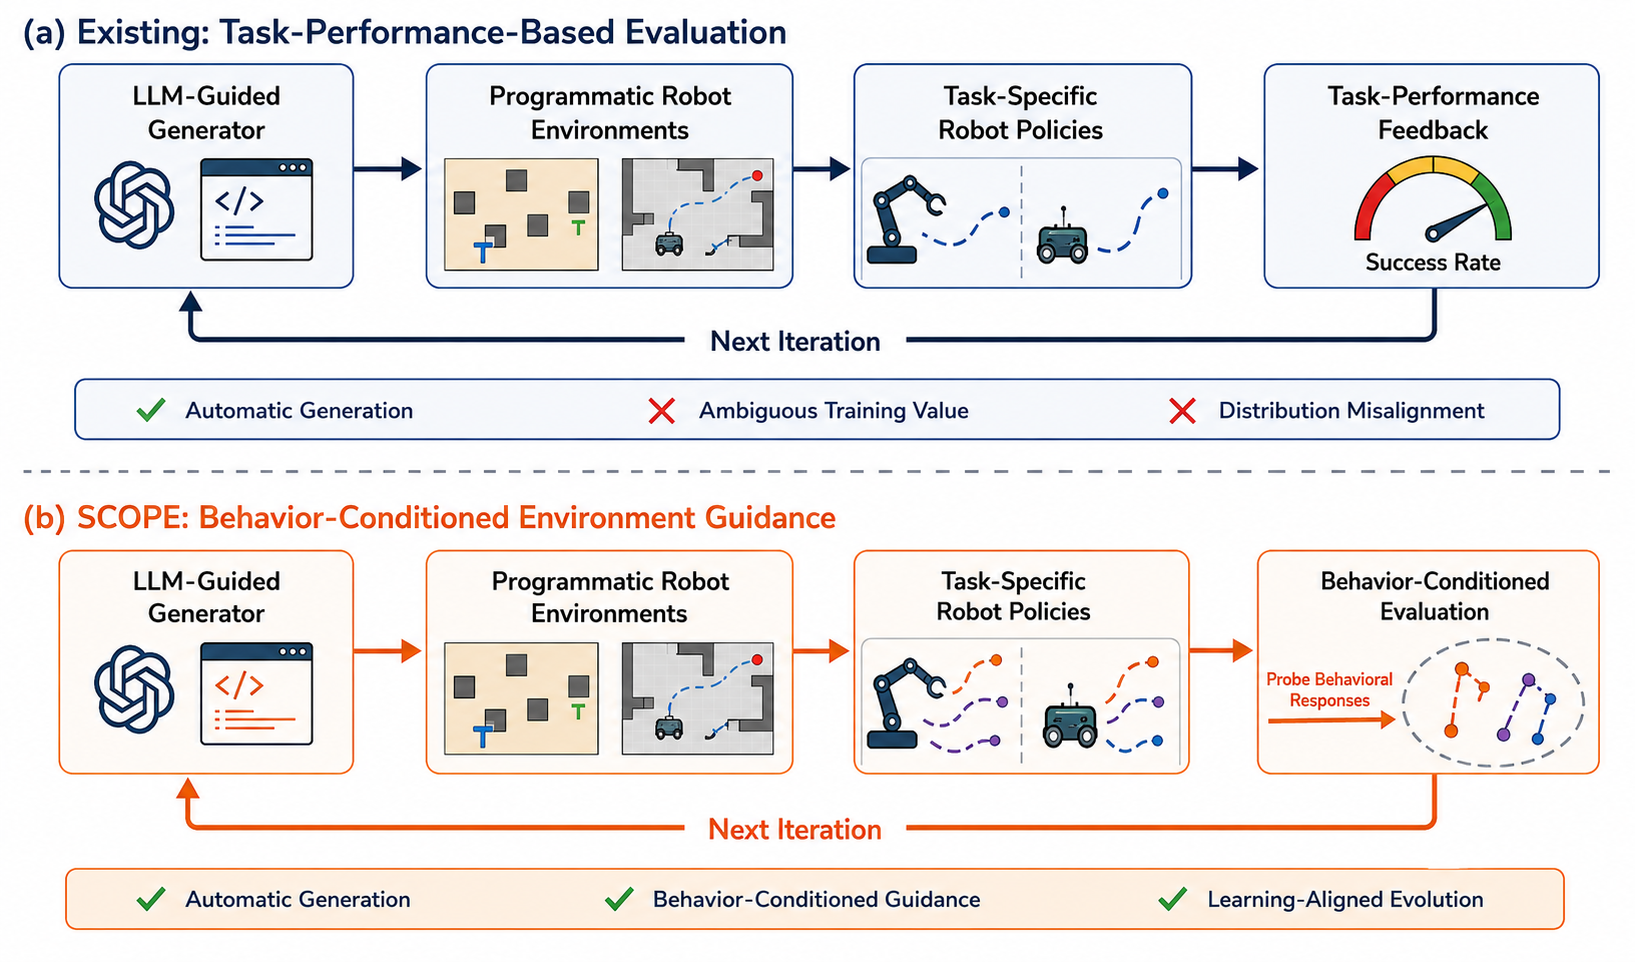
\includegraphics[width=\linewidth]{figures/figure1}
\caption{Comparison of feedback loops for programmatic environment generation.
(a) Existing methods use aggregate task-performance feedback to update an
LLM-guided generator, which can leave the training value of generated
environments ambiguous as the policy changes. (b) SCOPE probes generated
environments with the latent skill library and uses the resulting
skill-library-relative evaluation to guide the next generator update, coupling
training-distribution evolution to policy learning.}
\label{fig:intro}
\end{figure}

% =============================================================
\section{Introduction}
% =============================================================
Enabling robot policies to generalize reliably to unseen environmental
configurations remains a fundamental challenge in robot learning. Any finite
training process can expose a policy to only a subset of the configurations it
may encounter during deployment. The training distribution governs the
composition of this subset and thereby shapes the policy's generalization
behavior. Conventional approaches define this distribution through handcrafted
environmental priors~\cite{divo} or domain randomization over predefined
parameter spaces~\cite{tobin2017domain}. Specifying these priors and parameter
spaces requires substantial domain knowledge and task-specific tuning. Once
specified, however, these distributions typically remain fixed throughout
learning, despite continuing changes in the policy's capabilities and learning
requirements.

Large language models (LLMs) have exhibited robust capabilities in program
reasoning and code generation, substantially advancing the automated design of
training environments. Recent methods leverage these capabilities to synthesize
executable environment-generator programs from task specifications and
iteratively refine them using policy feedback, yielding families of training
environments without exhaustive manual enumeration of individual
scenes~\cite{eurekaverse,envgen,omniepic,curricullm}. This program-level
generation paradigm expands the scale and flexibility of training distribution
construction while making the resulting distributions revisable throughout
learning. Yet whether policy feedback provides a sufficiently informative basis
for directing this evolution as policy learning progresses remains unresolved.

Existing methods for policy-feedback-driven environment generation commonly
evaluate candidate environments using the current policy's task
performance~\cite{eurekaverse,envgen,curricullm}. Adaptive curriculum methods
further use regret, learning progress, or success variability to identify
environments that may remain useful for
training~\cite{paired,jiang2021plr,sfl}. Although these signals are constructed
differently, they ultimately summarize how each candidate environment relates
to the current policy at the task level. As policy learning progresses,
multiple candidate environments can receive identical or similar task-level
evaluations, causing the feedback to lose discrimination and provide limited
guidance for subsequent generator evolution.

Our key insight is that evaluating a candidate environment across the latent
skills of a shared policy~\cite{divo} exposes capability-conditioned differences
hidden by task-level summaries. Environments with the same task-level
evaluation can still be distinguished by the breadth of successful support they
receive from the current skill library. Success across all skills indicates
broad coverage by the learned repertoire, failure across all skills indicates
that the repertoire provides no successful response, and mixed outcomes
identify environments supported by only part of the current capabilities. We
formalize this capability-dependent relation between an environment and the
learned repertoire as \emph{skill-library-relative environment learnability}.
As policy learning reshapes the skill library, this reference evolves
accordingly, providing policy-dependent feedback for LLM-based evolution of the
training distribution.

To address this problem, we propose \textbf{SCOPE}
(\textbf{S}kill-Library-Guided \textbf{CO}evolution of \textbf{P}olicy and
\textbf{E}nvironment), which uses skill-library-relative feedback to evolve the
programmatic training distribution with the policy's capabilities. The main
contributions of this work are summarized as follows:
\begin{enumerate}
    \item We develop a closed-loop framework for
    Skill-Library-Guided Policy--Environment Coevolution that couples
    latent-skill policy learning with LLM-based programmatic environment
    generation, allowing acquired behavioral capabilities and the training
    distribution to evolve together.

    \item We introduce \emph{skill-library-relative environment learnability},
    a capability-dependent feedback signal derived from differences in task
    outcomes across the latent skills of a shared policy on each candidate
    environment. This signal guides generator-program evolution and
    interaction-based validation.

    \item We evaluate SCOPE on obstacle-constrained Push-T manipulation and
    navigation across diverse unseen environment distributions. The results
    demonstrate improved zero-shot generalization over baselines using manually
    designed training distributions, static LLM-generated environments, or
    curricula driven by aggregate task-performance feedback. Skill-conditioned
    trajectory and coevolution analyses further verify complementary behaviors
    and the effectiveness of the proposed feedback loop.
\end{enumerate}

% =============================================================
\section{Related Work}
% =============================================================
\textit{A. Large Language Models in Robot Learning}

Large language models have been applied to robot learning for semantic
planning, reward design, task generation, and executable program synthesis.
Leveraging their code-generation capabilities, Eureka synthesizes reward
functions from task descriptions, while DrEureka further constructs
domain-randomization configurations for sim-to-real
transfer~\cite{eureka,dreureka}. Beyond reward and parameter design, RoboGen
builds generative simulation pipelines for producing robot tasks, scenes, and
training data, whereas GenSim generates executable task code and demonstrations
that can be organized into a reusable task library~\cite{robogen,gensim}.
CurricuLLM uses LLM reasoning to decompose a complex robot-control problem into
an ordered curriculum of executable subtasks~\cite{curricullm}.

LLMs have also been used to construct or iteratively update policy-training
environments. OMNI-EPIC filters generated environment programs using
foundation-model judgments of learnability and
interestingness~\cite{omniepic}. Eurekaverse evolves terrain-generator
programs according to aggregate policy performance, while EnvGen modifies
environment configurations based on task-level statistics that identify the
skills an agent has yet to master~\cite{eurekaverse,envgen}. These methods rely
on different sources of feedback: foundation-model judgments need not track the
policy's evolving capabilities, whereas task-level statistics may lose
discrimination as policy performance saturates.

\textit{B. Environment Design and Curriculum Learning}

Training-distribution design has traditionally been studied through domain
randomization and curriculum learning. Domain randomization improves robustness
by training policies over predefined distributions of environmental
parameters~\cite{tobin2017domain}, but the resulting training distribution does
not respond to the learner's changing capabilities. Curriculum learning instead
organizes training tasks according to their difficulty or the learner's
progress~\cite{bengio2009curriculum,matiisen2020teacher,
portelas2020teacher}, allowing training to advance from currently accessible
tasks toward those requiring stronger capabilities.

Unsupervised environment design further automates curriculum construction by
generating and selecting environments relative to the current policy. PAIRED
formulates environment design as an adversarial game and searches for levels
that induce high regret between paired agents~\cite{paired}. PLR replaces a
learned environment generator with the prioritization and replay of randomly
sampled levels according to their estimated training
value~\cite{jiang2021plr}. ACCEL additionally mutates high-value levels,
allowing the curriculum to expand around the frontier of the learner's
capabilities~\cite{accel}. Subsequent analyses show that commonly used regret
approximations may track success-based learnability rather than regret itself,
motivating SFL to directly prioritize environments that are neither
consistently failed nor already mastered~\cite{sfl}. SFL estimates learnability
from outcome variability across repeated rollouts of the current policy. In
contrast, SCOPE evaluates matched outcomes across the latent-conditioned
behaviors of a shared policy, using their differential responses to characterize
skill-library capability coverage and guide programmatic generator evolution.
Collectively, these methods establish learner-relative environment evaluation
as a central principle of automatic curriculum construction.

\textit{C. Diverse Skill Learning}

Latent-conditioned policies provide a compact representation of multiple
behaviors within a shared model. Unsupervised skill-discovery methods differ
primarily in how they define behavioral diversity. DIAYN learns distinguishable
skills by maximizing the dependence between latent variables and visited
states, whereas DADS distinguishes skills according to their effects on state
transitions~\cite{diayn,dads}. These objectives promote broad behavioral
coverage without requiring task rewards, but the discovered behaviors are not
necessarily useful for solving a downstream task.

Task-directed methods therefore combine behavioral diversity with extrinsic
performance. LTD3 uses state--action-based mutual information to encourage
distinct solutions to the same task, while SMERL promotes diverse behaviors
subject to maintaining near-optimal task returns~\cite{ltd3,smerl}. In
obstacle-constrained manipulation, DIVO introduces random obstacles during
training to induce complementary task-solving behaviors, allowing the resulting
latent-skill policy to adapt to previously unseen obstacle
configurations~\cite{divo}.

SCOPE connects diverse skill learning with programmatic curriculum design by
recasting the learned skill repertoire from a policy-side representation of
diverse behaviors into a policy-relative basis for environment evaluation.
Capability coverage revealed by skill-conditioned responses then defines
environment learnability and guides the evolution of the training distribution.

% =============================================================
\section{Method}
\label{sec:method}
% =============================================================
We propose \textbf{SCOPE} (Skill-Library-Guided Coevolution of Policy and
Environment), a closed-loop framework that co-adapts a skill-conditioned robot
policy and the program that generates its training environments. At curriculum
iteration $t$, \emph{Stage~1} trains the shared policy on environments induced by
$g_t$ and probes its skill-conditioned behaviors to obtain the
response-annotated environment set $\mathcal R_t$ (Sec.~\ref{sec:signal}).
\emph{Stage~2} transforms this response profile and representative environments
into a structured evolution context $C_t$, from which an LLM proposes a set of
candidate generator programs $\mathcal G_t^{\mathrm{cand}}$
(Sec.~\ref{sec:generation}). \emph{Stage~3} compares the incumbent and candidate
generators under matched interaction conditions and adopts an eligible candidate
when supported by the skill-library responses; otherwise, $g_t$ is retained
(Sec.~\ref{sec:verification}). The selected $g_{t+1}$ defines the training
distribution for the next curriculum iteration, closing the loop in
Fig.~\ref{fig:overview}.

\begin{figure*}[t]
\centering
% \includegraphics[width=\textwidth]{figures/fig_overview}
\framebox[\textwidth][c]{\rule{0pt}{7.0cm}\ Fig.~2 placeholder: SCOPE framework overview (full-width)}
\caption{SCOPE co-evolution framework. At curriculum iteration $t$, Stage~1
trains the shared skill-conditioned policy on environments induced by $g_t$ and
extracts the response-annotated environment set $\mathcal R_t$. Stage~2
organizes the response profile and representative environments into the
structured evolution context $C_t$, from which the LLM proposes candidate
generator programs $\mathcal G_t^{\mathrm{cand}}$. Stage~3 compares the
incumbent and candidates under matched interaction conditions and either adopts
an eligible candidate or retains $g_t$. The resulting $g_{t+1}$ defines the
training distribution for the next curriculum iteration.}
\label{fig:overview}
\end{figure*}

% -------------------------------------------------------------
\subsection{Problem Formulation}
\label{sec:prelim}
\label{sec:problem}
% -------------------------------------------------------------
First, we model a fully specified environment as a finite-horizon Partially
Observable Markov Decision Process (POMDP),
\begin{equation}
 \mathcal{M}_e=
 \left(\mathcal{S},\mathcal{A},\mathcal{O},P_e,R,I,\gamma\right),
 \label{eq:pomdp}
\end{equation}
where $e=(s_0,c)\in\mathcal{E}$ denotes an environment configuration consisting
of an initial state $s_0$ and an obstacle configuration $c$;
$\mathcal{S}$, $\mathcal{A}$, and $\mathcal{O}$ are the state, action, and
observation spaces, respectively; $P_e:\mathcal{S}\times\mathcal{A}
\rightarrow\Delta(\mathcal{S})$ is the transition function under $e$;
$R:\mathcal{S}\times\mathcal{A}\rightarrow\mathbb{R}$ is the task reward;
$I:\mathcal{S}\rightarrow\mathcal{O}$ is the observation function; and
$\gamma\in[0,1)$ is the discount factor. Here, $\Delta(\cdot)$ denotes the space
of probability distributions over its argument.

An obstacle-generator program $g\in\mathcal{G}$ samples obstacle configurations
conditioned on the initial state,
\begin{equation}
 s_0\sim\mu_0,\qquad c\sim p_g(c\mid s_0),
 \label{eq:generator-distribution}
\end{equation}
and we denote the resulting distribution over environment configurations by
$p_g(e)$.

Let $\pi_\theta:\mathcal{O}\rightarrow\Delta(\mathcal{A})$ denote a policy
parameterized by $\theta$. Its expected discounted return in $\mathcal{M}_e$ is
\begin{equation}
 V^{\mathcal{M}_e}(\pi_\theta)=
 \mathbb{E}_{\tau\sim p(\tau\mid\mathcal{M}_e,\pi_\theta)}
 \left[\sum_{h=0}^{H-1}\gamma^h R(s_h,a_h)\right],
 \label{eq:environment-value}
\end{equation}
where $\tau$ denotes the interaction trajectory and $H$ is the episode horizon.

An environment curriculum is an ordered sequence of generator programs
\begin{equation}
 \mathbf{g}=(g_0,g_1,\ldots,g_T)\in\mathcal{G}^{T+1},
 \label{eq:generator-curriculum}
\end{equation}
where each $g_t$ induces a training distribution $p_{g_t}(e)$. Let
$\pi_{\mathbf{g}}$ denote the final policy obtained by sequentially training on
these distributions. Given a fixed task-success predicate
$\rho(\tau)\in\{0,1\}$ and an unseen test distribution $p_{\mathrm{test}}$, the
environment-curriculum design objective is
\begin{equation}
 \max_{\mathbf{g}\in\mathcal{G}^{T+1}}
 \mathbb{E}_{\substack{e\sim p_{\mathrm{test}}\\
 \tau\sim p(\tau\mid\mathcal{M}_e,\pi_{\mathbf{g}})}}
 \left[\rho(\tau)\right].
 \label{eq:curriculum-objective}
\end{equation}

% -------------------------------------------------------------
\subsection{Stage 1: Skill-Library Probing for Learnability Signal Extraction}
\label{sec:signal}
% -------------------------------------------------------------

\textbf{Skill-conditioned policy training.}
At curriculum iteration $t$, SCOPE trains a shared policy on the environment
distribution $p_{g_t}(e)$ induced by the current generator $g_t$. To generate
diverse actions, we define a skill set $\mathcal W=\{w_k\}_{k=0}^{K}$ and an
episode-level skill variable $w\in\mathcal W$.

Given the observation $o_h$ at step $h$, we extract a task-state representation
$x_h$ and encode the observation into an observation-dependent latent
representation $z_h$:
\begin{equation}
 x_h=\phi(o_h),
 \qquad
 z_h=E_\eta(o_h),
 \qquad
 z_h\in\mathcal Z,
 \label{eq:observation-latent}
\end{equation}
where $\mathcal Z$ denotes the latent representation space. The resulting
skill-conditioned policy is defined as
\begin{equation}
 \pi_\theta^w(a_h\mid o_h)
 \triangleq
 \pi_\xi(a_h\mid x_h,z_h,w),
 \qquad
 \theta=(\eta,\xi),
 \label{eq:skill-policy}
\end{equation}

Across training episodes, obstacle layouts sampled from $p_{g_t}(e)$ alter the
task constraints under which the skill-conditioned responses are learned. At
the beginning of each training episode, an environment $e\sim p_{g_t}(e)$ and a
skill variable $w\sim q(w)$ are sampled, where $q(w)$ is a fixed categorical
distribution over $\mathcal W$. The selected $w$ remains fixed throughout the
trajectory, whereas $z_h$ is updated from the current observation at every step.

Policy training under the current generator maximizes
\begin{equation}
 J_{\mathrm{task}}(\theta;g_t)
 =
 \mathbb E_{\substack{e\sim p_{g_t}(e)\\w\sim q(w)}}
 \left[
 V^{\mathcal M_e}\!\left(\pi_\theta^w\right)
 \right].
 \label{eq:generator-policy-objective}
\end{equation}
All skill conditions share the policy parameters and are jointly optimized on
the current environment distribution. After a fixed training interval, the
policy is held fixed for skill-library signal extraction.

\textbf{Skill-library signal extraction.}
Beyond policy optimization, skill-conditioned rollouts collected during probing
expose outcome variation across the behavioral modes of the current policy. To
localize its empirical capability boundary, we evaluate all skill conditions on
common scenes and extract a library-relative response signal.

After each training interval, we fix the resulting policy $\pi_{\theta_t}$ and
sample $M_c$ valid environments $\{e_i\}_{i=1}^{M_c}$ from the current generator
$g_t$. For each environment $e_i$, all $K$ skill conditions of the shared policy
are evaluated without exploration noise under the same initial state and
obstacle configuration. The trajectory and task outcome associated with skill
$w_k$ are defined as
\begin{equation}
 \begin{aligned}
  \tau_{ik}
  &\sim
  p\!\left(
  \tau\mid\mathcal M_{e_i},\pi_{\theta_t}^{w_k}
  \right),\\
  y_{ik}
  &\triangleq
  \rho(\tau_{ik})\in\{0,1\},
 \end{aligned}
 \label{eq:skill-conditioned-outcome}
\end{equation}
where $y_{ik}$ indicates whether the behavior conditioned on $w_k$ successfully
completes the task in $e_i$. We collect the outcomes across the skill library
into
\begin{equation}
 \mathbf y_i
 \triangleq
 \begin{bmatrix}
  y_{i1} & \cdots & y_{iK}
 \end{bmatrix}^{\!\top},
 \qquad
 \mathbf Y_t
 \triangleq
 \begin{bmatrix}
  \mathbf y_1^\top\\
  \vdots\\
  \mathbf y_{M_c}^\top
 \end{bmatrix}
 \in\{0,1\}^{M_c\times K}.
 \label{eq:skill-response-matrix}
\end{equation}
Here, $\mathbf y_i$ records the skill responses to environment $e_i$, while
$\mathbf Y_t$ forms the scene--skill response matrix over the sampled
environments.

We summarize the response of the skill library to $e_i$ by
\begin{equation}
 r_{\mathcal W}(e_i)
 \triangleq
 \frac{1}{K}\sum_{k=1}^{K}y_{ik}.
 \label{eq:skill-library-response}
\end{equation}
Although each rollout yields a binary task outcome,
$r_{\mathcal W}(e_i)\in\{0,1/K,\ldots,1\}$ provides a graded characterization of
the environment relative to the current skill library. A
\textbf{Skill-Selective} response is identified when the skill-conditioned
rollouts contain both successful and unsuccessful outcomes, equivalently,
$0<r_{\mathcal W}(e_i)<1$. This condition captures environments for which task
success depends on the conditioned behavior, thereby exposing the empirical
capability boundary of the current policy. Responses with
$r_{\mathcal W}(e_i)=0$ and $r_{\mathcal W}(e_i)=1$ are labeled \textbf{Unsolved}
and \textbf{Solved}, respectively.

Each sampled environment is annotated with its skill-response vector and
response rate, yielding the response-annotated environment set
\begin{equation}
 \mathcal R_t
 \triangleq
 \left\{
 \bigl(
 e_i,\mathbf y_i,r_{\mathcal W}(e_i)
 \bigr)
 \right\}_{i=1}^{M_c}.
 \label{eq:response-annotated-environments}
\end{equation}
The empirical distribution of $r_{\mathcal W}$ over $\mathcal R_t$ constitutes
the skill-library response profile of the current generator. This profile,
together with representative response-annotated environments, provides the
feedback for subsequent generator evolution.

% -------------------------------------------------------------
\subsection{Stage 2: Signal-Guided Generator Evolution}
\label{sec:generation}
% -------------------------------------------------------------

Given the response-annotated environment set $\mathcal R_t$, we transform
skill-library feedback into a structured context for evolving the current
generator and its induced training distribution.

\textbf{Signal-conditioned context construction.}
Let $m_t^{\mathrm U}$ and $m_t^{\mathrm S}$ denote the empirical proportions of
\textbf{Unsolved} and \textbf{Solved} environments in $\mathcal R_t$,
respectively. Given a fixed saturation threshold
$\eta_{\mathrm{sat}}>1/2$, we set the evolution direction $d_t$ to
\textsc{Relax} when $m_t^{\mathrm U}\geq\eta_{\mathrm{sat}}$,
\textsc{Harden} when $m_t^{\mathrm S}\geq\eta_{\mathrm{sat}}$, and
\textsc{Diversify} otherwise. The \textsc{Diversify} direction instructs the LLM
to preserve the current Skill-Selective coverage while exploring alternative
environment structures.

For each evolution direction, we select a fixed number of representative
environments from the relevant response regions. The direction $d_t$,
representative environment descriptions, and their skill responses
$\bigl(\mathbf y_i,r_{\mathcal W}(e_i)\bigr)$, together with the current
generator $g_t$, are organized into a structured evolution context $C_t$. This
context specifies the desired distributional change and grounds generator
evolution in concrete environment structures associated with the current
response profile.

\textbf{LLM-guided generator evolution.}
Conditioned on $C_t$, we independently sample $N_{\mathrm{cand}}$ candidate
generator programs from the LLM:
\begin{equation}
 \begin{aligned}
  g_t^{(j)}
  &\sim p_{\mathrm{LLM}}\!\left(\,\cdot\mid C_t\right),
  &&j=1,\ldots,N_{\mathrm{cand}},\\
  \mathcal G_t^{\mathrm{cand}}
  &\triangleq
  \left\{g_t^{(j)}\right\}_{j=1}^{N_{\mathrm{cand}}}.
 \end{aligned}
 \label{eq:candidate-generators}
\end{equation}
Sampling multiple candidates allows the method to consider alternative
adaptations under the same evolution objective and reduces reliance on any
single LLM generation. Each executable candidate represents a stochastic
generator rather than an individual environment instance and therefore induces
an environment distribution $p_{g_t^{(j)}}(e)$. The resulting candidates are
subsequently evaluated through policy--environment interaction to determine
whether any candidate should replace $g_t$.

% -------------------------------------------------------------
\subsection{Stage 3: Interaction-Validated Generator Update}
\label{sec:verification}
% -------------------------------------------------------------
Given the candidate set $\mathcal G_t^{\mathrm{cand}}$, we determine whether the
proposed changes to the induced environment distribution are supported by
policy--environment interaction. Executability alone does not establish the
curriculum value of a candidate generator. We therefore compare the incumbent
and candidate generators under matched probing conditions before updating the
curriculum.

\textbf{Paired interaction validation.}
We sample $M_v$ initial states and hold them fixed across all generators under
comparison. For every generator
$g\in\{g_t\}\cup\mathcal G_t^{\mathrm{cand}}$, the generator produces an
environment $e_\ell^g$ for each initial state, and all skill conditions in
$\mathcal W$ are evaluated using the fixed policy $\pi_{\theta_t}$. The initial
states, policy, and skill library are shared across generators, whereas each
generator induces its own obstacle configurations and interaction trajectories.
This paired design controls variation in the probing conditions and enables a
more direct comparison of the induced environment distributions.

Before response-based comparison, candidates must pass basic feasibility checks
for executability, valid environment generation, and non-degeneracy. For each
generator under comparison, we reuse the response rate $r_{\mathcal W}$ and
define its Skill-Selective coverage under the fixed validation budget as
\begin{equation}
 n_t^{\mathrm{sel}}(g)
 \triangleq
 \#\Bigl\{
 \ell\ \Big|\ 
 e_\ell^g\ \text{is valid},\
 0<r_{\mathcal W}(e_\ell^g)<1
 \Bigr\}.
 \label{eq:skill-selective-coverage}
\end{equation}
Because all generators are evaluated using the same $M_v$ initial states,
$n_t^{\mathrm{sel}}(g)$ provides a policy-relative criterion for generator
comparison. We additionally compute the empirical proportions of
\textbf{Unsolved} and \textbf{Solved} responses among the valid validation
environments generated by each generator.

\textbf{Validation-gated generator update.}
Candidate eligibility is determined relative to the incumbent response profile.
A candidate is eligible when it passes the feasibility checks and improves
$n_t^{\mathrm{sel}}$ by a prespecified margin. To prevent the curriculum from
remaining at a saturated endpoint, direction-consistent candidates may also be
admitted. Under \textsc{Relax}, a candidate should reduce the Unsolved proportion
without increasing the Solved proportion beyond a prescribed tolerance. Under
\textsc{Harden}, it should reduce the Solved proportion without increasing the
Unsolved proportion beyond the corresponding tolerance.

Under \textsc{Diversify}, the LLM is encouraged to explore alternative
environment structures during candidate generation. The validation gate
preserves policy-relative curriculum value by requiring a candidate to retain
Skill-Selective coverage within a prescribed tolerance while preventing an
excessive increase in the Solved proportion. Structural exploration is therefore
induced during candidate generation rather than treated as an interaction-derived
validation score. The margins and tolerances are fixed throughout training and
reported in the experimental setup.

Among the candidates satisfying the corresponding feasibility and response-based
criteria, we select the one with the largest $n_t^{\mathrm{sel}}$ to define
$g_{t+1}$. If no candidate satisfies these criteria, the incumbent generator is
retained, i.e., $g_{t+1}=g_t$. Consequently, an LLM-proposed evolution changes
the training distribution only when it satisfies the interaction-based adoption
criterion. The resulting $g_{t+1}$ defines the environment distribution for the
next training interval, completing the closed-loop evolution of the policy and
its training environments.

\begin{algorithm}[H]
\caption{SCOPE Coevolution Procedure}
\label{alg:scope}
\small
\begin{algorithmic}[1]
\Require Coding LLM; task specification and generator contract; skill library
$\mathcal W$ and sampling distribution $q$; evolution rounds $T$; budgets
$M_c$, $M_v$, and $N_{\mathrm{cand}}$; saturation threshold
$\eta_{\mathrm{sat}}$; fixed validation margins and tolerances
\Ensure Final policy $\pi_\theta$ and generator curriculum
$\mathbf g=(g_0,\ldots,g_T)$
\State Initialize policy parameters $\theta$
\State $g_0 \gets \Call{SynthesizeGenerator}{\text{task},\text{contract}}$
\For{$t=0,\ldots,T$}
    \Statex \textit{Stage 1: Policy training and skill-library probing}
    \State $\theta \gets
    \Call{TrainPolicy}{\theta,p_{g_t},\mathcal W,q}$
    \If{$t=T$}
        \State \textbf{break}
    \EndIf
    \State $\mathcal R_t \gets
    \Call{ProbeSkillLibrary}{\pi_\theta,g_t,\mathcal W,M_c}$
    \Statex \textit{Stage 2: Signal-guided generator evolution}
    \State $d_t \gets
    \Call{SelectDirection}{\mathcal R_t,\eta_{\mathrm{sat}}}$
    \State $C_t \gets
    \Call{ConstructContext}{g_t,d_t,\mathcal R_t}$
    \State $\mathcal G_t^{\mathrm{cand}} \gets
    \Call{LLMCandidates}{C_t,N_{\mathrm{cand}}}$
    \Statex \textit{Stage 3: Interaction-validated generator update}
    \State $\mathcal G_t^{\mathrm{feas}} \gets
    \Call{FeasibilityFilter}{\mathcal G_t^{\mathrm{cand}}}$
    \State $\mathcal J_t \gets
    \Call{InteractionValidate}{\pi_\theta,\mathcal W,g_t,
    \mathcal G_t^{\mathrm{feas}},d_t,M_v}$
    \If{$\mathcal J_t\neq\varnothing$}
        \State $j^\star\in
        \arg\max_{j\in\mathcal J_t}
        n_t^{\mathrm{sel}}(g_t^{(j)})$
        \State $g_{t+1}\gets g_t^{(j^\star)}$
    \Else
        \State $g_{t+1}\gets g_t$
    \EndIf
\EndFor
\State \Return $\pi_\theta$ and $\mathbf g$
\end{algorithmic}
\end{algorithm}

% =============================================================
\section{Experiments}
\label{sec:exp}
% =============================================================
Our experiments target three questions. \textbf{Q1:} Does a learnability-driven
LLM curriculum improve zero-shot generalization over hand-designed, static, and
single-policy-feedback baselines? \textbf{Q2:} Does the skill-library signal
remain informative where single-policy feedback degenerates? \textbf{Q3:} Is the
gain attributable to the \emph{signal source} rather than to LLM generation
itself?

\subsection{Setup}
\textbf{Tasks and policy.} We evaluate Push-T obstacle manipulation in
MuJoCo~\cite{todorov2012mujoco} and Point-agent navigation in Safety-Gymnasium.
The training distribution contains exactly two fixed-size static obstacles in
both tasks: boxes in Push-T and pillars in navigation. We use a DIVO stage-1
latent policy~\cite{divo} trained with TD3~\cite{td3}.
The initial generator $g_0$ is produced by an LLM and evolved by SCOPE, which
samples $N_{\mathrm{cand}}$ candidate programs per cycle. The LLM backend,
prompt, skill-sampling distribution $q(w)$, $K$, $M_c$, $M_v$,
$N_{\mathrm{cand}}$, $\eta_{\mathrm{sat}}$, and all validation margins and
tolerances are reported for reproducibility.

\textbf{No-leakage protocol.} The best checkpoint is selected on a \emph{fixed}
validation distribution that is independent of the evolving $g_t$ and disjoint
from the test distributions, so no test information enters model selection.

\textbf{Held-out distributions.} Final generalization is measured on four held-out
obstacle distributions unseen during training: Big (B), Multiple (M),
Unstructured (U), and Dynamic (D). B changes obstacle count and size, M uses
three obstacles instead of the two seen during training, U changes obstacle
shape and topology, and D introduces time-varying obstacles. The two tasks share
these abstract factors but use task-specific realizations. In particular,
Push-T relocates obstacles between policy steps, whereas navigation uses
phase-offset continuously moving Gremlins whose relative geometry changes over time.
For navigation we also evaluate a matched frozen
control, $D_{\mathrm{static}}$, with identical geometry, starts, and seeds. We
report $D_{\mathrm{static}}-D$ as the dynamic drop, but do not include the
control as a fifth term in the B/M/U/D average.

\textbf{Baselines.} We compare (a) a manual ``between'' rule with exactly two
standard static obstacles; in navigation, the start is chosen so that one of
the two obstacles lies between the agent and goal, (b) a static generator with no online update,
(c) a single-policy-feedback curriculum that drives the same LLM loop with the
deployed policy's success instead of the skill-library signal, and (d) SCOPE
(ours). Arms (b)--(d) start from the same LLM-generated $g_0$ and differ only in
the feedback source and whether the generator evolves, so any difference isolates
the contribution rather than a change of initial distribution.

\textbf{Metrics.} We report zero-shot success rate on B/M/U/D and its average,
and the matched dynamic drop for navigation;
skill-library statistics ($\realized$, $\lv$, $\bcount$); and, for diversity, the
effective number of skills and within/across-scene trajectory diversity. The
effective number of skills is
$N_{\mathrm{eff}}\!=\!\exp\!\big(-\sum_k \alpha_k\log \alpha_k\big)$, where
$\alpha_k$ is the fraction of solved probe scenes attributed to skill $w_k$;
$N_{\mathrm{eff}}\!=\!K$ indicates that all skills contribute equally and
$N_{\mathrm{eff}}\!\to\!1$ indicates collapse onto a single behavior. Trajectory
diversity is the mean pairwise distance between the object paths of different
skills on a shared scene (within-scene) and of the same skill across scenes
(across-scene), so that a high $N_{\mathrm{eff}}$ reflects genuinely distinct
behaviors rather than relabeled copies.

\subsection{Zero-Shot Generalization (Q1)}
Table~\ref{tab:heldout} reports preliminary Push-T zero-shot success on the
held-out distributions. Navigation uses the same B/M/U/D factors defined above;
its multi-seed results are \todo{run and add}.
% NOTE: preliminary, single seed; replace with >=3 seeds and fill arm (c).
SCOPE attains the highest average and improves most on the hardest dynamic
distribution, where the static generator collapses. These numbers are preliminary
and single-seed; the multi-seed comparison and the single-policy-curriculum arm
(c) are \todo{run and fill}.

\begin{table}[t]
\caption{Push-T zero-shot success rate on Big (B), Multiple (M), Unstructured
(U), and Dynamic (D) held-out distributions (preliminary, single seed;
multi-seed, navigation results, and arm (c) to be added).}
\label{tab:heldout}
\centering
\begin{tabular}{lccccc}
\toprule
Method & B & M & U & D & Avg \\
\midrule
Manual (between)          & 0.42 & 0.30 & 0.53 & 0.10 & 0.34 \\
Static generator          & 0.53 & 0.65 & 0.85 & 0.05 & 0.52 \\
Single-policy curriculum  & \multicolumn{5}{c}{\todo{run}} \\
SCOPE (ours)              & \textbf{0.60} & \textbf{0.75} & \textbf{0.90} & \textbf{0.18} & \textbf{0.61} \\
\bottomrule
\end{tabular}
\end{table}

\subsection{The Signal Does Not Degenerate at Maturity (Q2)}
Across evolution rounds, deployment success saturates: train-time and
deployed-skill probe success reach $0.93$--$1.00$. Over the same rounds the
skill-library $\realized$ stays in the range $0.2$--$0.48$ with a spread across scenes
(Fig.~\ref{fig:decoupling}). Single-policy feedback thus becomes uninformative
(everywhere ``solved'') while the library signal remains rankable---the effect
our design exploits. We further report the coverage of obstacle placements over
rounds to confirm that the accepted generators do not collapse the layout
distribution into a trivial spike \todo{fill coverage curve}.

\begin{figure}[t]
\centering
\framebox[\linewidth][c]{\rule{0pt}{3.0cm}\ Fig.~2 placeholder: decoupling curve}
\caption{Decoupling over evolution rounds: deployment success saturates near
$1.0$, while skill-library $\realized$ remains in $0.2$--$0.48$ with a
cross-scene spread, so a rankable learnability signal persists after the
single-policy signal has collapsed.}
\label{fig:decoupling}
\end{figure}

\subsection{Cost of Single-Stage Bare Deployment}
Because we deploy a single skill rather than searching the library at test time,
we quantify the cost of this choice. Table~\ref{tab:gap} reports, per obstacle
size, the best-library-skill solvability ($\feasible$ level), the library
$\realized$, and single-skill deployment success. The gap between the best skill
and deployment is $2.5$--$5\%$, indicating that keeping the library as a lens
rather than deploying it costs little, which supports the single-stage design.

\begin{table}[t]
\caption{Solvability vs.\ obstacle size (preliminary).}
\label{tab:gap}
\centering
\begin{tabular}{ccccc}
\toprule
Size & feasible & realized & deployed & gap \\
\midrule
0.01 & 1.000 & 0.379 & 0.975 & 0.025 \\
0.05 & 1.000 & 0.392 & 0.950 & 0.050 \\
0.08 & 0.900 & 0.279 & 0.875 & 0.025 \\
\bottomrule
\end{tabular}
\end{table}

\subsection{Ablations (Q3) --- Protocol}
The decisive test of our claim is the \emph{feedback-source} ablation: holding the
LLM, the generator interface, the validator, and $g_0$ fixed, we replace the
skill-library signal with a single-policy success signal and compare held-out
generalization. We additionally ablate the probe size $K\!\in\!\{4,8,16\}$; the
saturation escape (on/off); and the single-primary-score validator against a multi-axis
``not-worse'' variant, measuring both held-out success and the number of accepted
updates before the curriculum stalls. Results are \todo{run and report}; the
expected outcome is that (d) exceeds the single-policy arm and that removing the
saturation escape induces the maturity stall described in
Sec.~\ref{sec:verification}.

\subsection{Skill Diversity and Qualitative Analysis}
To verify that the probe library is genuinely diverse rather than collapsed, we
report the effective number of skills and within/across-scene trajectory
diversity \todo{fill}. Qualitatively, we overlay the trajectories of the $K$
skills on a single layout and the deployed trajectory on held-out scenes,
illustrating detour behaviors on B/M/U and the failure modes that make D hard
\todo{add qualitative figure}.

% =============================================================
\section{Conclusion and Limitations}
% =============================================================
We presented SCOPE, which measures learnability across a skill library to recover a
graded, rankable curriculum signal in the deterministic zero-shot regime where
single-policy feedback degenerates, and uses it to drive a non-ratcheting LLM
generate--verify loop over obstacle-generator programs. The evaluation protocol
instantiates the same held-out factors on Push-T and navigation with
task-specific obstacle dynamics. Preliminary Push-T results show improved
held-out success and a decoupling between deployment success and skill-library
learnability that motivates the design; the navigation results remain to be
completed.

\emph{Limitations.} The skill library is a measurement lens and is never deployed;
whether training a diverse library benefits single-skill deployment beyond a
shared decoder is a hypothesis we test rather than assume. Deployment success can
saturate within the training obstacle size, so harder held-out distributions are
needed to expose the generalization gap. The present results are preliminary and
single-seed; the multi-seed four-arm comparison and the ablations in
Sec.~\ref{sec:exp} are required to establish that the library signal outperforms
single-policy feedback, and are the focus of ongoing work.

\textbf{AI-usage disclosure.} An LLM is a component of the proposed method
(generator evolution) and was also used to assist manuscript editing; all
technical claims and results were produced and verified by the authors.

\bibliographystyle{IEEEtran}
\bibliography{references}

\end{document}
